\documentclass[11pt,a4paper]{article}

\usepackage{amsmath}
\usepackage{amssymb}
\usepackage{amsthm}
\usepackage{tikz}
\usetikzlibrary{shapes,arrows}
\usepackage{hyperref}

\title{Guidance Navigation and Control}
\author{AUT}
\date{Informal lecture notes for week 37, 2019}


\tikzstyle{block} = [draw, rectangle, minimum width=6em]
\tikzstyle{sum} = [draw, fill=blue!20, circle, node distance=1cm]
\tikzstyle{input} = [coordinate]
\tikzstyle{output} = [coordinate]
\tikzstyle{pinstyle} = [pin edge={to-,thin,black}]

\newtheorem{definition}{Definition}


\begin{document}
\maketitle
\section{State estimation problem}

We divide the state estimation problem in three blocks
\begin{enumerate}
	\item Formal representation of the states of our system
	\item Modeling the dynamics of our states (predictions)
	\item Particular example: Discrete Kalman Filter
\end{enumerate}

\section{Formal representation of the states of our system}
We represent the states of our system with a vector $q$ containing as elements \emph{probability density functions} (or \emph{pdf} for short) instead of containing real numbers. We employ such representation because the \emph{pdf} contains information about the uncertainty that we might have on a property of the system, whereas a simple real number cannot encode such information. Therefore, we represent the states of our system with the column vector $q = \begin{bmatrix} f_1 & f_2 & \dots & f_n \end{bmatrix}^T$, where $n$ is the number of states of the system, and $f_n$ are the different \emph{pdfs} (to be defined shortly) associated to each of our states.

Let us define the \emph{pdf} as $f(\cdot) := \mathcal{V} \to \mathbb{R}_+$, where $\mathcal{V}$ is the space where state of interest belongs to, for example, a position $p_x\in\mathbb{R}$ in meters or temperature $\theta\in\mathbb{R}_+$ in Kelvins, and the output of $f(\cdot)$ is always positive. The \emph{pdf} is giving us the information about the probability of a random variable to be between two values. Therefore the probability of having the random variable between $-\infty$ and $\infty$ is $1$ (or informally $100\%$). We can write this fact formally as follows
\begin{equation}
\operatorname{Prob}[x\in (-\infty,\infty)] := \int_{-\infty}^{\infty} f(x) dx = 1.
	\label{eq: fus}
\end{equation}
Note that $\operatorname{Prob}[x\in (a,a)] = 0, \, a\in\mathbb{R}$ if $f(x)$ is 
\emph{smooth enough}.

There exist many different \emph{pdf} depending on the nature of the variable and its uncertainty, such as \emph{uniform}, \emph{normal}, \emph{exponential}, etc. You can click on this link to find information about them \url{https://www.statlect.com/probability-distributions/}.

We are interested in two properties of the \emph{pdf}. The first one is the expected value, or $E[x] = \hat x$, where
\begin{equation}
	E[x] = \int_{-\infty}^{\infty} f(x)\, x \,dx, \label{eq: ep}
\end{equation}
where if $f(x)$ is symmetric, then $\hat x$ is the center point of such symmetry.

The second property is the \emph{variance}, which is a particular case of the \emph{covariance} $CoVar[x,y] := E[(x-\hat x)(y-\hat y)]$. The variance is calculated when we set $x=y$, then it measures the expected squared \emph{distance} of your random variable to its expected value. This is also known as $\sigma_x^2$, and note that obviously is a non-negative number. In fact, $\sigma_x^2$ is a positive number for a generic distribution. If you consider $\sigma_x^2 = 0$, then it must be true that  $\operatorname{Prob}[x\in (\hat x,\hat x)] = 1$, which does not hold in general, at least not for the \emph{uniform} or the \emph{normal pdf}.

\subsection{Simple fusion algorithm}
If you have $n$ \emph{pdf} from $n\in\mathbb{N}$ {\bf uncorrelated sources} referring to the same state, then you can fuse them as follows
\begin{equation}
	\operatorname{Prob}[x\in (-\infty,\infty)] = \frac{1}{\alpha}\int_{-\infty}^{\infty} \prod_n f_n(x) \, dx = 1, \label{eq: fus}
\end{equation}
where $\alpha\in\mathbb{R}_+$ is a positive scaling factor to calculate such that we have $1$ as a total probability. Therefore, if we would like to calculate the probability of finding $x\in(a_1,a_2)$, then
\begin{equation}
	\operatorname{Prob}[x\in (a_1,a_2)] = \frac{1}{\alpha}\int_{a_1}^{a_2} \prod_n f_n(x) \, dx. \label{eq: pro}
\end{equation}
Note that the expression (\ref{eq: pro}) is valid for any generic \emph{pdf}. Furthermore, they can be different in nature like $f_1$ is \emph{uniform} and $f_2$ \emph{normal}.

Of course, if you want to find out the expected value after the fusion, you must apply the definition in (\ref{eq: ep})
\begin{equation}
	E[x] = \int_{-\infty}^{\infty} \frac{1}{a}\prod_n f_n(x)\, x \,dx,
\end{equation}
and the same for the variance. These two operations can be very demanding numerically (computational power). That will motivate the study of the following \emph{normal probability density function}.

\subsection{\emph{Normal pdf}}
The \emph{normal pdf} is a popular function that approximates very well many natural phenomena, and we are lucky that it is tractable mathematically. Specially when we are \emph{fusioning} different normal \emph{pdf}, and when these normal \emph{pdf} goes through linear transformations, e.g., a linear dynamics for a model.

Let us define the normal \emph{pdf} as
\begin{equation}
	g(x) = \frac{1}{\sqrt{2\pi\sigma_x^2}}\operatorname{exp}\left[\frac{(x-\hat x)^2}{2\sigma_x^2}\right],
\end{equation}
where we plot it in Figure \ref{fig: gauss}. Note that $g(x)$ is characterized uniquely by two parameters, the expected value $\hat x$ and the variance $\sigma^2_x$.

\begin{figure}
\centering
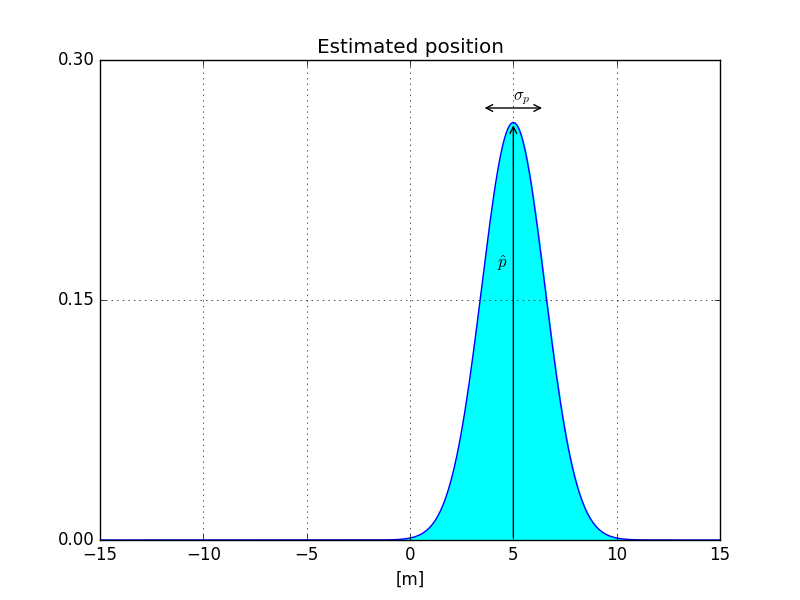
\includegraphics[scale=0.5]{./images/pdf_pos.png}
\caption{Normal probability density function, with $\hat p$ being the expected position of a vehicle in the $x$ axis, and $\sigma_p$ being the standard deviation calculated from the variance $\sigma_p^2$. The range $\hat p \pm \sigma_p$ includes the 68\% of all the values in the distribution approximately.}
\label{fig: gauss}
\end{figure}

\subsection{Sensor fusion of two normal \emph{pdf}}
According to (\ref{eq: fus}) we can fuse two normal \emph{pdf}, if they come from independent sources, as follows
\begin{equation}
g_f(x) = g_1(x)g_2(x),
\end{equation}
which is an easy operation since we are dealing with exponentials. In particular, we have that $g_f(x)$ is characterized by
\begin{equation}
	\begin{cases}
		\hat x_f &= \frac{\hat x_1\sigma_{x_2}^2 + \hat x_2\sigma_{x_1}^2 }{\sigma_{x_1}^2 + \sigma_{x_2}^2} \\
		\sigma_f^2 &= \frac{\sigma_{x_1}^2 \sigma_{x_2}^2}{\sigma_{x_1}^2 + \sigma_{x_2}^2}
	\end{cases}.
	\label{eq: fusg}
\end{equation}
Note that we just derived the Kalman gain from the famous Kalman filter. If we define $k := \frac{\sigma_{x_1}^2}{\sigma_{x_1}^2 + \sigma_{x_2}^2}$ then we can rewrite (\ref{eq: fusg}) as
\begin{equation}
	\begin{cases}
		\hat x_f &= \hat x_1 + k(\hat x_2 - \hat x_1) \\
		\sigma_f^2 &= \sigma_1^2 - k\sigma_1^2
	\end{cases}.
	\label{eq: fusg2}
\end{equation}

The normal \emph{pdf} is a particular case of a \emph{Pearson distribution} \url{https://en.wikipedia.org/wiki/Pearson_distribution}, and expressions (or nice approximations) like (\ref{eq: fusg}) can be found for other distributions as well.

\section{Modeling the dynamics of our states. Linear systems and normal \emph{pdfs}}
If we represent our states with real numbers, it is common to find the equations that predict the evolution of our states at different fixed time intervals (discrete time) as
\begin{equation}
	q(k+1) = f(q(k),u(k)),
	\label{eq: st}
\end{equation}
where $k\in\mathbb{N}$ is the time event, $q\in\mathbb{R}^n$ (with $n\in\mathbb{N}$ being the number of states), $u\in\mathbb{R}^p$ (with $n\in\mathbb{N}$ being the number of inputs), and $f := \mathbb{R}^n\times\mathbb{R}^p \to \mathbb{R}^n$ being the \emph{state-transition} function. If we can write (\ref{eq: st}) as a linear system, i.e.,
\begin{equation}
	q(k+1) = F q(k) + G u(k),
	\label{eq: st2}
\end{equation}
with $F\in\mathbb{R}^{n\times n}$ and $G\in\mathbb{R}^{n \times p}$, then we have very good news when the elements of $q$ are not real numbers but normal \emph{pdfs}. In particular, linear combinations (as in (\ref{eq: st2})) of normal \emph{pdfs} have as a result another normal \emph{pdf}, check this link for the proof \url{https://www.statlect.com/probability-distributions/normal-distribution-linear-combinations}. {\bf That is not the case in general for arbitrary \emph{pdf}s.} One nice consequence of this fact is that if we take a normal distribution $g_f$ that is a linear combination of other normal distributions $g_n$, then the expected value of $g_f$ is also the same linear combination of the expected values from $g_n$, i.e,
\begin{equation}
\hat q(k+1) = F \hat q(k) + G \hat u(k),
	\label{eq: st3}
\end{equation}
so we can reuse $F$ and $G$ from (\ref{eq: st2})!

Remember that a normal distribution is characterized by its expected value $\hat x$ and variance $\sigma_x^2$. Then, together with (\ref{eq: st3}) we need to find out the evolution of the variances of the considered normal distributions. Consider the following \emph{covariance} matrix for your vectorial state $q$
\begin{equation}
	P := CoVar(q,q) := \begin{bmatrix}
		CoVar(q_1,q_1) & \dots & CoVar(q_1,q_n) \\
		\vdots & \ddots & \vdots \\
		CoVar(q_n,q_1) & \dots & CoVar(q_n,q_n)
	\end{bmatrix} = E[(q-\hat q)(q-\hat q)^T].
\end{equation}
Note that by definition we have that $\sigma_{q_n}^2 = CoVar(q_n,q_n)$, so the diagonal elements are the covariances of the states in $q$.

Now we check the following identity for the vector $q$ and a matrix $F$.
\begin{align}
	CoVar(Fq,Fq) &= E[(Fq-F\hat q)(Fq-F\hat q)^T] \nonumber \\
	&= E[F(q-\hat q)(q -\hat q)^TF^T] \nonumber \\
	&= F E[(q-\hat q)(q -\hat q)^T] F^T \nonumber \\
	&= F \, CoVar(q,q) \, F^T = F P F^T \label{eq: cool}
\end{align}
Note that $F$ is a constant matrix, and all constants can get out of the integral (\ref{eq: ep}) for calculating expected values. That is why the last step in (\ref{eq: cool}).

Now let us calculate
\begin{align}
	CoVar(q(k+1), q(k+1)) = CoVar(Fq(k)+Gu(k),Fq(k)+Gu(k)).
	\label{eq: co2}
\end{align}
From the definition we can check that the covariance of the linear combination of two variables is given by
\begin{equation}
	CoVar(ax + by) = a^2\,CoVar(x,x) + b^2\, CoVar(y,y) + 2ab \, CoVar(x,y).
\end{equation}
The covariance $CoVar(x,y) = 0$ means that $x$ and $y$ are not correlated, i.e., if we assume that $q(k)$ and $u(k)$ are not correlated (state and input at the same time instant are independent of each other), then we can continue (\ref{eq: co2}) as
\begin{align}
	P(k+1) &= CoVar(Fq(k)+Gu(k),Fq(k)+Gu(k)) \nonumber \\
	&= CoVar(Fq(k),Fq(k)) + CoVar(Gu(k),Gu(k)) \nonumber \\
	&= FP(k)F^T + G\,CoVar(u(k),u(k))\,G^T. \nonumber \\
	&= FP(k)F^T + GQ(k)G^T\label{eq: Pk}
\end{align}

Note that $Q$ in (\ref{eq: Pk}) is a diagonal matrix if there are no correlations between the inputs. The diagonal elements of $Q$ are just $\sigma^2_{u_i}, i\in\{1,\dots,p\}$. Therefore, we can predict the evolution in (discrete) time of a normal distribution by iterating (\ref{eq: st2}) for the expected value of $q$ and (\ref{eq: Pk}) for the variance of $q$.

\section{Measurements. Inputs \& observations in linear systems}
Equations (\ref{eq: st3}) and (\ref{eq: Pk}) indicate how the \emph{pdf}'s associated to the states $q$ evolve \textbf{if} the \emph{pdf}'s are normal, and the process that we consider can be modelled as a linear system. Therefore, we can make predictions over time starting from an initial \emph{pdf}. In particular from the initials $\hat q(0)$ and $P(0)$.

We can employ measurements for both, to make predictions and to improve/update the information that carries our \emph{pdf}. If the measurements are employed to predict in (\ref{eq: st}), then they are considered \emph{inputs}. If the measurements are compared with a prediction, then they are considered as \emph{observations}.

If we only consider inputs, then the uncertainty of the input $u$ will increase the uncertainty of our states in $q$ each time we iterate (\ref{eq: Pk}). The observations can be employed to improve our estimation of the \emph{pdfs} associated with $q$ by following \emph{sensor fusion} as in (\ref{eq: fusg}) or (\ref{eq: fusg2}). When we fuse two sources of information, we must ensure they represent the same quantity, for example, they are both velocities and they are in the same units.

Example of observation: We might measure a velocity employing a pressure sensor, which is proportional to the square of the velocity. Consider, $q = \begin{bmatrix} p_x & v_x & b_a \end{bmatrix}^T$, where $p_x$ is a position, $v_x$ is a velocity and $b_a$ is a bias from an accelerometer. Then the \emph{observation function} that gives the squared velocity will be
\begin{equation}
y = h(q) = v_x^2 \neq H q.
\label{eq: hnl}
\end{equation}
We call $y\in\mathbb{R}$ the \emph{predicted observation} (it might be a vector of course), which will be fused with the actual measurement later on. However, we note that (\ref{eq: hnl}) cannot be written as a function of a matrix $H\in\mathbb{R}^{1\times 3}$ multiplying the state $q$. Therefore, (\ref{eq: hnl}) is said to be \emph{nonlinear}. We are interested in \emph{linear observation functions} since we know that the following holds for normal \emph{pdf}'s.
\begin{equation}
\hat y = H \hat q,
\end{equation}
i.e., the predicted observation is also a normal $\emph{pdf}$, and its associated covariance
\begin{equation}
	P_y = CoVar(Hq, Hq) = HPH^T.
\end{equation}
The actual measurement must be also associated to a $\emph{pdf}$, therefore it will be described by the corresponding $\hat y_m$ and $P_{y_m}$. The covariance matrix $P_{y_m}$ is also known as $R$ in the literature, the \emph{measurement noise}.

\subsection{Sensor fusion. Kalman gain}
Let us rewrite again (\ref{eq: fusg}) and (\ref{eq: fusg2})

\begin{equation}
	\begin{cases}
		\hat x_f &= \frac{\hat x_1\sigma_{x_2}^2 + \hat x_2\sigma_{x_1}^2 }{\sigma_{x_1}^2 + \sigma_{x_2}^2} \\
		\sigma_f^2 &= \frac{\sigma_{x_1}^2 \sigma_{x_2}^2}{\sigma_{x_1}^2 + \sigma_{x_2}^2}
	\end{cases}.
	\label{eq: fusgbis}
\end{equation}
\begin{equation}
	\begin{cases}
		\hat x_f &= \hat x_1 + k(\hat x_2 - \hat x_1) \\
		\sigma_f^2 &= \sigma_{x_1}^2 - k\sigma_{x_1}^2
	\end{cases},
	\label{eq: fusg2bis}
\end{equation}
where $k = \frac{\sigma_{x_1}^2}{\sigma_{x_1}^2 + \sigma_{x_2}^2}$. These (\ref{eq: fusgbis}) and (\ref{eq: fusg2bis}) have been derived for the unidimensional case, i.e., we fused two normal \emph{pdf}'s. Now $\hat q$ is a vector, and $P$ is a matrix, instead of $\hat x$ and $\sigma_x^2$. Let us consider the subscript $1$ as our prediction, and $2$ as our measurement to extend (\ref{eq: fusg2bis}) in matrix form. We first note that $\sigma_{x_1}^2$ would be extended to $P_y = HPH^T$ and $\sigma_{x_2}^2$ would be extended to $P_{y_m}$. Therefore we can extend $k$ as
\begin{equation}
K = HPH^T (P_y + P_{y_m})^{-1},
\end{equation}
so we can extend the second equation in (\ref{eq: fusg2bis}) as
\begin{align}
	HP_fH^T &= HPH^T -  HPH^T (P_y + P_{y_m})^{-1} HPH^T,
	\label{eq: e}
\end{align}
and noting that we are multiplying by $H$ and $H^T$ at the right and left-hand sides of each term in (\ref{eq: e}), then we have that
\begin{align}
	P_f &= P - PH^T(P_y + P_{y_m})^{-1} HP \nonumber \\
	P_f &= P - KHP. \label{eq: Pf}
\end{align}
Thus, we can extend easily (\ref{eq: fusg2bis}) to matrix form the fused mean for the state $q$ as
\begin{equation}
	\hat q_f = \hat q_1 + K(\hat y - \hat y_m).
	\label{eq: qf}
\end{equation}
The equations (\ref{eq: Pf}) and (\ref{eq: qf}) are typically known as the \emph{correction} step in a Kalman filter.

\end{document}
